\documentclass[12pt,a4paper,titlepage,onecolumn]{article}
\usepackage[latin1]{inputenc}
\usepackage{amsmath}
\usepackage{amsfonts}
\usepackage{amssymb}
\usepackage{graphicx}
\usepackage{titlesec}
\newcommand{\sectionbreak}{\clearpage}
\author{mkem114 - 6273632}
\title{VOXSpell User Manual}

\begin{document}
	\maketitle
	\tableofcontents
	\listoffigures
	
	\section{Getting Started}
	You might need an adult to help you get started the first time. You need open a terminal; change to the game folder(if not already there), type in "chmod 777 RUN.sh" (without the quote marks), press enter, type in "./RUN.sh" and press enter. Please see Figure ~\ref{fig:TerminalandFolder} for a general look, the green and blue writing is normally different for you as well as the icons and theme.
	\begin{figure}[h]
	\centering
	\includegraphics[width=1\linewidth]{"Figures/Getting Started/TerminalandFolder"}
	\caption[Terminal commands]{General overview of terminal, commands and folder with VOXSpell}
	\label{fig:TerminalandFolder}
	\end{figure}\\
	Please read the "README.txt" as and if there's any problems it may help.
	
	\section{Introduction}
	Welcome to VOXSpell! The best spelling quiz game for New Zealand kids! If you haven't already read the README.txt file please do because it's important.\\
		\subsection{Quitting/Exiting}
		If your parents, teacher or caregiver catch you playing when you're not meant to be or if you're done playing exit the game at any time by pressing the little "X" button normally in the top-right or top-left corners of VOXSpell like in Figure ~\ref{fig:Exit}.
		\begin{figure}[h]
		\centering
		
\includegraphics[width=0.1\linewidth]{Figures/Introduction/Exit}
		\caption[Quit/Exit]{VOXSpell quit/exit button}
		\label{fig:Exit}
		\end{figure}
		\subsection{To Main Menu}
		Most of the time a button called "Menu" will be in the bottom-right corner of VOXSpell that will take you to the main menu if you click on it (see Figure ~\ref{fig:Menu}).
		\begin{figure}[h]
		\centering
		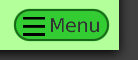
\includegraphics[width=0.2\linewidth]{Figures/Introduction/Menu}
		\caption[Menu Button]{Menu button always goes to the main menu}
		\label{fig:Menu}
		\end{figure}


	
	\section{Picking a Level}
	\begin{figure}[h]
	\centering
	\includegraphics[width=1\linewidth]{"Figures/Picking a Level/PickLevelGeneral"}
	\caption[PickLevel]{First run (and reset) screen to pick starting level}
	\label{fig:PickLevelGeneral}
	\end{figure}

	When you run VOXSpell for the first time you will see something like Figure ~\ref{fig:PickLevelGeneral}. This is because you need a level to start from, you should pick a level that isn't too hard and not too easy for you. \\
	You can pick a level by clicking where it says "1" in Figure ~\ref{fig:PickLevelGeneral} and then clicking on the name of the level that you would like to pick. If you would like to hear a word in the level to find out how hard it is then click on the "Preview" button as in Figure ~\ref{fig:PickLevelGeneral}.\\
	Once you picked the level you want to start on click on the "Play" button which will take you to the main menu.
	
	\section{Main Menu}
	\begin{figure}[h]
	\centering
	\includegraphics[width=1\linewidth]{"Figures/Main Menu/MainMenuGeneral"}
	\caption[Main Menu]{The main menu}
	\label{fig:MainMenuGeneral}
	\end{figure}
	After a level has been picked or if the game is run again (not for the first time) then this screen like in Figure ~\ref{fig:MainMenuGeneral} will appear; this is the main menu. To play a new quiz click on the "Play" button. To play any level or add your own levels or your own words click on the "Custom" button. To see your game scores click on "Statistics". To change the voice or reset the game click on the "Options" button. 
	\subsection{Background Music}
	To pause the background music that plays everytime you go to the main menu click on the "Music" button and to start it playing it again click on "Music" again. When you leave the main menu the music stops playing so you can hear the speaker. To change the music look in the README.txt
	
	\section{Playing a Quiz}

	\section{Playing a Custom Quiz}
		
	\section{Viewing Statistics}
		\subsection{Levels}
		\subsection{Sorting}
		
	\section{Changing Options}
		\subsection{Voices}
		\subsection{Reset}
		
\end{document}